\section*{Zielsetzung}
Das Ziel dieses Versuchs ist die Bestimmung der Compton-Wellenlänge $\lambda_c$ des Elektrons
\section{Theorie}
\label{sec:Theorie}
\subsection{Röntgenstrahlung}
Die Röntgenstrahlung wird hier in einer evakuierten Röntgenröhre erzeugt.
In dieser werden mit einer Glühkathode freie Elektronen erzeugt, die dann zu der positiv geladenen Anode hin beschleunigt werden.
Durch das Auftreffen der Elektronen auf die Anode und dem Abbremsen dieser im Coloumbfeld der Anodenatome, entsteht ein Bremsspektrum. Bei dieser Abbremsung wird ein Photon (Röntgenquant) ausgesendet, welches die Energie besitzt, die das abgebremste Elektron verloren hat.
Außerdem wird das Anodenmaterial durch die Elektronen ionisiert,
sodass dieses ebenfalls Photonen emittieren kann, wenn ein Elektron aus einer äußeren Schale in eine innere zurückfällt.
In diesem Fall ist die Energie des Photons gerade
die Energiedifferenz der beiden Energieniveaus. Daher besteht das charakteristische Spektrum des Anodenmaterials aus festen Linien, deren Energie charakteristisch für das Anodenmaterial der
Röntgenröhre ist. \newline

\noindent Die Absorption von Photonen durch Materie einer bestimmten Dicke d kann durch das Delamber´sche Gesetz
\begin{equation}
    I = I_0 \cdot \exp{(-\mu d)} 
\end{equation}
beschrieben werden, wobei $I_0$ die einfallende Intensität darstellt.
\noindent Der Absorptionskoeffizient setzt sich aus den Koeffizienten verschiedener Effekte nach
\begin{equation}
    \mu = \mu_\text{Photo} + \mu_\text{Paar} + \mu_\text{Com}
\end{equation}
zusammen, dabei beziehen sich die Absorptionskoeffizienten auf den Photoeffekt, die Paarbildung und den Comptoneffekt.
\subsection{Bragg Reflexion}
Mit der Bragg-Reflexion kann die Wellenlänge der Röntgenstrahlung untersucht werden.
    \begin{figure}[H]
       \centering
        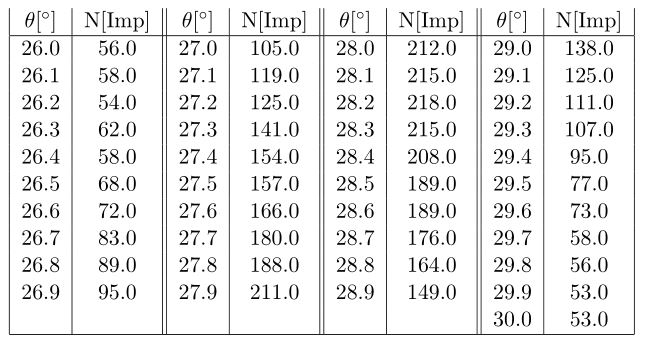
\includegraphics[width=0.3\textwidth]{images/bragg.jpg}
        \caption{Bragg-Reflexion der Röntgenstrahlung an einem Kristallgitter. \cite{603}}
       \label{fig:bragg}
    \end{figure}
    \noindent
    Wie in \autoref{fig:bragg} zu sehen ist, wird die Röntgenstrahlung an einem Kristallgitter gebeugt, sodass die Strahlen bei einem Glanzwinkel $\alpha$ konstruktiv interferieren
    und die gebeugte Wellenlänge in n-ter Beugungsordnung mit der Bragg-Bedingung
    \begin{equation}
        2d \sin{\alpha} = n \lambda
        \label{eqn:bragg}
    \end{equation}
    berechnet werden kann.

\subsection{Compton-Effekt}
Es hat sich experimentell gezeigt, dass sich die Wellenlänge von $\gamma$-Strahlung bei Streuung an einem Elektron zu längeren Wellenlängen verschiebt. Dieser Effekt wird auch als Compton-Effekt bezeichnet. In diesem Versuch wird die Compton-Wellenlänge mit Hilfe von Röntgenstrahlen bestimmt. Dazu werden die Röntgenstrahlen an einem Plexiglasquader gestreut, um aus dem Transmissionsverhalten die Comptonwellenlänge zu bestimmmen. 
\newline
\noindent
Bei der Compton Streuung wechselwirkt ein Photon mit einem freien Elektron und gibt einen
Teil seiner Energie an das Elektron ab, wobei es um den Winkel $\theta$ gestreut wird. Dieser Vorgang ist schematisch in \autoref{fig:compton} dargestellt.
\begin{figure}[H]
    \centering
     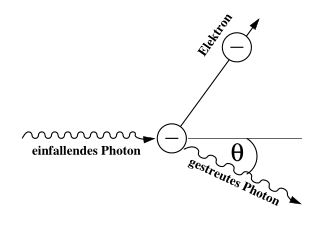
\includegraphics[width=0.6\textwidth]{images/compton.jpg}
     \caption{Photon und Elektron beim Compton-Effekt. \cite{603}}
    \label{fig:compton}
 \end{figure}
 \noindent
 Dabei verändert sich die Wellenlänge des Photons um $\symup{\Delta}\lambda = \lambda_2 - \lambda_1$ mit einfallender Wellenlänge $\lambda_1$ und Compton verschobener Wellenlänge $\lambda_2$. Aus der
 Energie- und Impulserhaltung erhält man für die Wellenlängendifferenz:
 \begin{equation}
    \symup{\Delta}\lambda = \frac{h}{m_\text{e} c}(1 - \cos{\theta})
    \label{eqn:wellenl}
\end{equation} 
\noindent
Wie zu erkennen ist, wird $\symup{\Delta}\lambda$ für $\theta = \SI{0}{\degree}$ mit $\symup{\Delta}\lambda = 0$ minimal und für $\theta = \SI{180}{\degree}$ mit $\symup{\Delta}\lambda = 2(\sfrac{h}{m_\text{e}c})= 2\lambda_\text{c}$ maximal. 
Die konstante Länge $\lambda_\text{c} = \frac{h}{m_\text{e}c}$ wird auch Compton-Wellenlänge des Elektrons genannt.